
\section{Results}
\label{sec:results}

We have developed a set of benchmark applications to evaluate the efficacy of the \acp{SNN}.
These benchmarks are presented in Table \ref{table:benchmarks}, and the code is available publicly at \textit{https://github.com/PRETgroup/ssann}. 
All benchmarks were written in Esterel and C, and the enforcers implemented according to~\cite{recps}.


Benchmarks include: an \acf{AV} braking system, described in Section \ref{sec:case}; an \acf{ESS} inspired by~\cite{chaudhari2017hybrid}; and a simple, two-team, zero-sum game called RABBIT.
The \ac{ESS} (described in Section~\ref{sec:ess}) has two different policies; ensuring that the system battery's \ac{SoC} never drops too low or rises too high  ($\varphi_{soc}$) and ensuring that the power by which the battery is charging or discharging is never too high ($\varphi_{charge}$).
RABBIT (described in Section~\ref{sec:rabbit}) has two policies, one policy ensures that the players never move out of the game's bounds ($\varphi_{bound}$), and the other policy ensures that all players do not make decisions that would result in loss of score ($\varphi_{score}$) (or opportunity to gain score) thus ensuring more successes for both teams.
%These examples all include various \acp{SNN} arrangements that use \acp{MLP} as the \acp{SANN}, however the \ac{AV} system is the only system to use deep \acp{ANN} in the form of \acp{CNN} in addition to \acp{MLP}.
Each benchmarks are analysed with and without \ac{RE} in place, to show the improvement in each system's safety when using \ac{RE}.
Additionally, the overhead generated by each enforcer is also calculated using measurement based timing on each system. 
Table~\ref{table:policies} lists every policy and provides a brief overview of each policy and it's measured overhead.
As can be seen, the overhead of the combined policies was less than 5\% for \ac{ESS} and RABBIT; these systems both had relatively simple and small enforcers.
The overhead for the \ac{AV} combined policy was less than 10\%, but this policy had a lot more safety conditions to enforce than either of the other two systems. 

% Benchmarks
\begin{table}[b]
	\centering
	\caption{Benchmarks and descriptions}
	\label{table:benchmarks}
	\begin{tabular}{@{}|l|l|l|l|@{}}
		\hline
		Name & \ac{SANN} Type(s) & \#\acp{SANN} & \#Enforced Policies \\ \hline
		\acs{AV} & \ac{MLP}, \ac{CNN}  & 28 & 4 \\
		\acs{ESS} & \ac{MLP} & 3 & 2 \\
		RABBIT & \ac{MLP}  & 6 & 2 \\
		\hline
	\end{tabular}
\end{table}

\begin{table}[t]
	\centering
	\caption{Design and overhead of the policies used in \ac{ESS}, \ac{AV} and RABBIT}
	\label{table:policies}
	\begin{tabular}{|p{0.25\linewidth}|p{0.06\linewidth}|p{0.12\linewidth}|p{0.06\linewidth}|p{0.11\linewidth}|p{0.1\linewidth}|}
		\hline Policy & States & Transitions & Timed & Execution Time (us) & Overhead (\%) \\ \hline
		\multicolumn{6}{|p{0.70\linewidth}|}{\ac{ESS}} \\ \hline 
		$None$ 										& N/A & N/A & N/A & 2.70 & 0 \\ 	
		$\varphi_{soc}$    							& 1 & 7 & No & 2.836 & 4.9 \\
		$\varphi_{charge}$    						& 1 & 4 & No & 2.71 & 0.346 \\
		$\varphi_{soc} \wedge \varphi_{charge}$  	& 1 & 11 & No & 2.84 & 4.935 \\ \hline       
		\multicolumn{6}{|p{0.70\linewidth}|}{\ac{AV}} \\ \hline
		$None$ 						&  &  &  & 736 & 0 \\
		$\varphi_{cnn}$ 			& 1 & 15 & No & 764 & 3.8 \\
		$\varphi_{drive}$ 			& 1 & 4 & No & 740 & 0.54 \\
		$\varphi_{car}$ 			& 1 & 7 & No & 774 & 5.1 \\
		$\varphi_{ped}$ 			& 2 & 56 & Yes & 767 & 4.2 \\
		$\varphi_{cnn} \wedge \varphi_{drive} \wedge \varphi_{car} \wedge \varphi_{ped}$ 	
		& 2 & 99 & Yes & 803 & 9.1 \\ \hline       
		\multicolumn{6}{|p{0.70\linewidth}|}{RABBIT} \\ \hline
		$None$ 										&  &  &  & 90.1 & 0 \\ 
		$\varphi_{bound}$ 							& 2 & 16 & No & 89.45 & -0.7 \\
		$\varphi_{score}$ 							& 2 & 112 & Yes & 94 & 4.3 \\
		$\varphi_{bound} \wedge \varphi_{score}$ 	& 2 & 126 & Yes & 93.8 & 4.1 \\ \hline      
	\end{tabular}
\end{table}

\subsection{\acf{ESS}} \label{sec:ess}
The \ac{ESS} is inspired by \cite{chaudhari2017hybrid}, in which an \ac{EV} charging station has a separate battery that it uses to assist the charging of the \acp{EV}, with the general idea that the battery is charged when power is cheap, and discharged when demand is high or power is expensive.
The \ac{ESS} uses a three-layer \ac{MLP} to decide the action for the battery in the next tick.
%The overall output of this \ac{MLP} is whether the battery is charging or discharging, and how much power it is charging or discharging.
%Since the ideal outputs of the \ac{ESS} are unknown, the \ac{ESS} controller was trained using a type of reinforcement learning called Q-learning~\cite{qlearning2010}.
%While the \ac{AV} system is a hard real-time system the \ac{ESS} system is a soft real-time system, as a missed deadline won't result in fatalities.
%Failures in this system could cause damage to electrical components and potentially cause fires (from overcharging or overcurrents) and maybe even customer property, i.e. the charging station and the \acp{EV}, and thus appropriate policies can be put into place to make the system safer.
Even though this system's \ac{MLP} was well-trained (via Q-learning~\cite{qlearning2010}), and tests of it only showed safe behaviour (it never outputted dangerous commands that could have overcharged the battery or allowed for an overcurrent discharge to occur), it is very difficult for testing to be fully comprehensive of any system.
Hence, \ac{SRE} can be used to formally guarantee that the controller will behave safely at all times.
%This allows us to show that even though the system has been well trained and hardly even makes mistakes, \ac{SRE} can still be used to improve the system's safety without affecting the performance of the system.
%The enforced policies monitor the controller's \ac{MLP} outputs and ensure that (1) the battery levels never reach critical levels, and (2) that too much power is never given or taken from the battery in too short a period of time.
%Running this system with enforced policies shows that the battery's \ac{SoC} never exceeds critical values and that the battery never charges or discharges too much power.
%The charge of buying and selling electricity to the customer's \ac{EV} does not change by any significant amount when the enforcer is in place, i.e. it does not affect the performance of the system while it keeps the system safe.customer's
The results of the system with and without the policies enforced are shown in Table~\ref{table:essres}, while the policies' structure and overhead are shown in Table~\ref{table:policies}.

% Ess results
\begin{table}[t]
	\centering
	\caption{Comparison of ESS with and without enforced policies}
	\label{table:essres}
	\begin{tabular}{|p{0.4\linewidth}|p{0.12\linewidth}|p{0.12\linewidth}|p{0.12\linewidth}|}
		\hline Enforcer used & No enforcer &  Enforcer & Ideal \\ \hline
		Times high charge/discharge power was detected & 52 & 0 & 0 \\ \hline      
		Lowest battery \ac{SoC} & 0.21 & 0.25 & 0.25 \\ \hline
		Minutes of critically low \ac{SoC} & 87 & 0 & 0 \\ \hline
		Highest battery \ac{SoC} & 0.905 & 0.905 & 0.95 \\ \hline
		Minutes of critically high \ac{SoC} & 0 & 0 & 0 \\ \hline
		Daily cost of buying power (\$) & 335 & 336 & < 380 \\ \hline 
	\end{tabular}
\end{table}

\subsection{\acf{AV}}
The \acp{ANN} in this system were trained for varying amounts of epochs, notably 1, 10, 100, 1,000, 10,000 and 100,000 epochs.
A partially trained \ac{ANN} will exhibit behaviour that is unexpected, and perhaps unsafe, because \acp{ANN} gain robustness through training, i.e. a less trained \ac{ANN} will be less robust.
This partially trained system is used to show how \ac{SRE} can prevent unsafe events in a system that does not behave as expected.

The \ac{AV} system's performance was measured by the amount of time the \ac{AV} was able to run before a accident occurred within the system.
At every level of training, the whole system was run 10,000 times, where one run consisted of running the system for 100 ticks, noting if and when an accident occurred and what caused the accident. 
Figure~\ref{fig:avtrained} compares the amount of training of the \ac{AV} system's \acp{ANN} with the performance of the system at that amount of training, as measured by the average number of ticks the system ran for before an unsafe incident occurred.
As expected, there is a direct relationship between the amount of training and the duration before an accident occurred, the difference between a less trained and more trained system is noticeable.
However, the difference between a less trained and more trained system is almost unnoticeable when the system has enforced policies. 

Over-training is a well known phenomenon that \acp{ANN} suffer. 
Over-training occurs when \acp{ANN} become too well trained on the data set they are trained with and, as a result, perform poorly on extrapolated data sets. 
Over-training was observed in the \ac{AV} system.
After approximately 10,000 epochs of training, the performance of the system began to drop. 
Due to the nature of the training algorithm and the data used, the system began to make more unsafe decisions in lieu of increasing the average speed of the vehicle.
However, the results also showed that the enforced system behaved just as safely when over-trained as it did under-trained, or even perfectly trained. 
This has applicability in many autonomous systems, where the ideal amount of training for the system is unknown. 

Few accidents were noted when the system used \ac{RE}, and the few accidents that did occur were the result of a vehicle hitting the \ac{AV} from behind when it slammed on the brakes to avoid a collision in front of it.
As seen in Table~\ref{table:avenf}, the enforcer not only reduced the number of accidents, but also reduced the speed of the vehicle to safe levels. 
An additional measure of performance was the percentage of brake actions the vehicle took that were unnecessary, i.e. brake actions when there were no obstacles on the road or pedestrians in sight.

\begin{table}[h]
	\centering
	\caption{Results of the AV system with and without the enforced policies}
	\label{table:avenf}
	\begin{tabular}{|p{0.15\linewidth}|p{0.15\linewidth}|p{0.15\linewidth}|p{0.15\linewidth}|p{0.15\linewidth}|}
		\hline Number of epochs trained & Percentage accidents & Average minutes to first accident per day & Average speed (km/h) & Percentage bad brakes \\ \hline
		\multicolumn{5}{|p{0.75\linewidth}|}{Not enforced} \\ \hline
		0 & 100	 & 3.21 & 98 & 19 \\ \hline
		1 & 100 & 3.3 & 93 & 19 \\ \hline
		10 & 100 & 3.8 & 81 & 57 \\ \hline
		100 & 100 & 5.35 & 59 & 24 \\ \hline
		1000 & 100 & 5.31 & 58 & 27 \\  \hline
		10000 & 48.5 & 73.9 & 18 & 63 \\ \hline
		100000 & 91.5 & 39 & 31.5 & 65 \\ \hline 
		\multicolumn{5}{|p{0.75\linewidth}|}{Enforced} \\ \hline
		0 & 75.7 & 75.6 & 45 & 0.7 \\ \hline 
		1 & 70.2 & 82.8 & 47 & 4.2 \\ \hline 
		10 & 88.5 & 58.9 & 37 & 20 \\ \hline 
		100 & 79.5 & 72.6 & 41 & 17 \\ \hline 
		1000 & 80.5 & 71.0 & 40 & 18 \\ \hline 
		10000 & 64 & 97.07 & 27.5 & 27 \\ \hline   
		100000 & 57 & 97.14 & 29 & 28 \\ \hline                  
	\end{tabular}
\end{table}

%\begin{figure}[t]
%	\centering
%	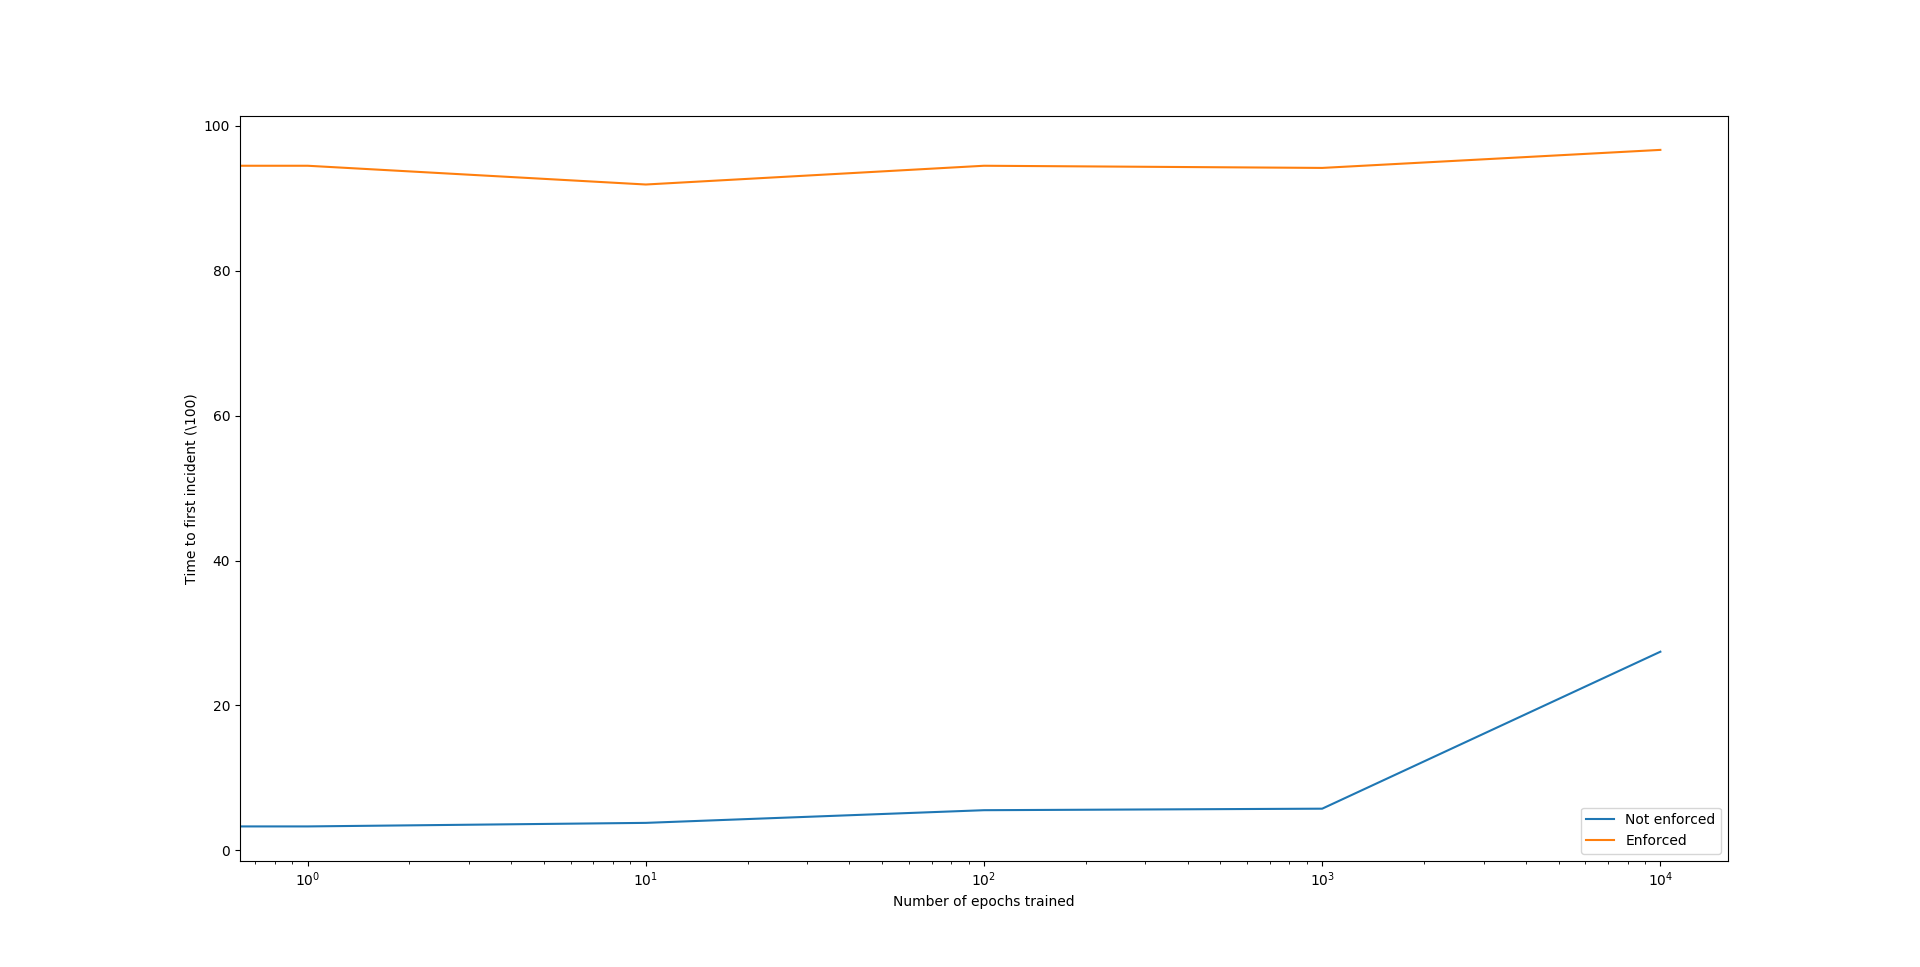
\includegraphics[width=\linewidth]{fig/AV-trained.png}
%	\caption{Graph showing the performance of the AV system with and without the enforcer with different lengths of \ac{ANN} training.	\label{fig:avtrained} \todo{Graph is completely useless, make fonts bigger, draw using pgfplots?}}
%\end{figure}
\begin{figure}[t]
	\centering
	\includegraphics[width=\linewidth]{avgraph.tikz}
	\caption{Graph showing the performance of the AV system with and without the enforcer with different lengths of \ac{ANN} training. \label{fig:avtrained}}
\end{figure}

\subsection{RABBIT} \label{sec:rabbit}
RABBIT is a simple game that is played between two teams: a team with one rabbit on it, and an opposing team with two wolves. 
The goal of the game differs for the two teams; the rabbit must make it safely off the playing field using a rabbit hole, while the wolves need to try reach the rabbit before it escapes.
%The playing field is an $m\times{n}$ matrix, where each coordinate is a possible position that each animal could move in to.
%The rabbit holes are place on the game boundary, i.e. the edges of the matrix.
Each animal is controlled using a single \ac{ANN} that decides, based on the animal's "vision", into which adjacent space the animal is moving to next.
%The \acp{ANN} were trained using reinforcement learning, as the ideal actions of each animal in any given state were unknown, there are simply too many states to compute that.
RABBIT has no safety implications to humans, as it is a game played between two teams of \ac{AI}, but policies can be enforced to increase the efficiency of the animals and reduce the errors made by the animals.
The policies ensure that the animals never leave the playing field, and that their movements are more refined, e.g. not getting stuck in one place, not moving away from their objective, etc.
The results of the policies are shown in Table~\ref{table:rabbitres}, and the structure and overhead of these policies are described in Table~\ref{table:policies}.

% Rabbit results
\begin{table}[h]
	\centering
	\caption{Comparison of RABBIT system with and without enforced policies}
	\label{table:rabbitres}
	\begin{tabular}{|p{0.2\linewidth}|p{0.2\linewidth}|p{0.2\linewidth}|p{0.2\linewidth}|}
		\hline Enforced & Rabbit wins (\%) &  Wolves wins (\%) & Neither animal wins (\%) \\ \hline
		No & 3 & 17 & 80 \\
		Yes & 36 & 59 & 5 \\ \hline       
	\end{tabular}
\end{table}
